\newpage
{\samepage
\begin{center}
{\Large{\bf Binary Trees}}
\end{center}
\begin{itemize}
\item Binary trees are used extensively in computer science
\item Game Trees
\item Searching
\item Sorting
\end{itemize}
\begin{center}
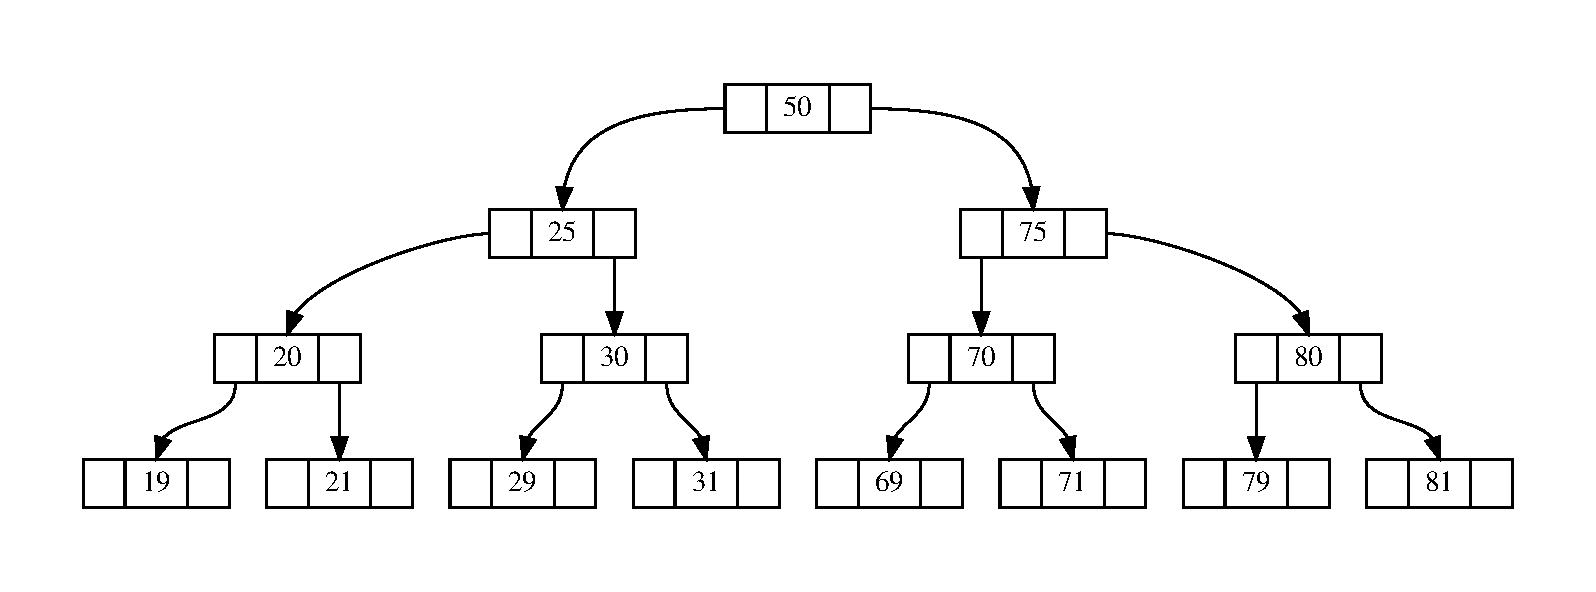
\includegraphics[width=\textwidth]{../Images/Linkedb.pdf}
\end{center}
}

\newpage
{\samepage
\begin{center}
{\Large{\bf Nomenclature}}
\end{center}
\begin{itemize}
\item Trees drawn upside-down !
\item Ancestor relationships: A is the parent of E
\item Can refer to left and right children
\item In a tree, there is only one path from the root to any child
\item A node with no children is a leaf
\item Most trees need to be created dynamically
\item Empty subtrees are set to NULL
\end{itemize}
\begin{verbatim}
typedef struct Node {
   char letter;
   struct Node *left;
   struct Node *right;
}
\end{verbatim}
}

\newpage
{\samepage
\begin{center}
{\Large{\bf Binary Trees\\[1.75ex]{\small(via an Array)}}}
\end{center}
Don't rush to assume a linked data structure must be used to implement
trees. You could use $1$ cell of an array for the first node, the next
two cells for its children, the next $4$ cells for their children and
so on. You need to mark which cells are in use \& which aren't ...
Counting from cell $1$:
